\chapter{Oblique Shocks}
\section{Recap}
\subsection{Analogy with hydraulic jumps}
"Supersonic flows" in the kitchen. In free-surface flows, we have the Froude number
\begin{gather}
    Fr = \dfrac{u}{c}
\end{gather}
\begin{itemize}[noitemsep]
    \item $Fr < 1$: subcritical
    \item $Fr > 1$: supercritical
    \item $u$: (depth averaged) flow speed
    \item $c$: wave speed
\end{itemize}
Understanding these flows are important for looking at forces on buildings/bridges. The same conservation principles apply (except energy; which is not conserved here) and is equivalent to $\delta = 2$. Used by Ernest Mach to illustrate shock collision with walls.
\subsection{Oblique shocks and terminology}
The Mach number varies with position in space. Shock represents:
\begin{enumerate}
    \item change in stagnation pressure
\end{enumerate}
and depends on
\begin{enumerate}
    \setcounter{enumi}{1}
    \item stagnation pressure unchanged
    \item rapid changes over a short distance
\end{enumerate}
\begin{itemize}[noitemsep]
    \item Oblique shock - flow is deflected and squashed.
    \item Weak oblique shocks (Mach number is supersonic on both sides).
    \item Strong oblique shock (Mach number is subsonic after shock)
\end{itemize}
\subsection{Streamlines}
The local \textbf{instantaneous} velocity $u(x,t)$ is tangential to the local streamline. Streamlines have directions and need arrows!
\begin{figure}[H]
    \centering
    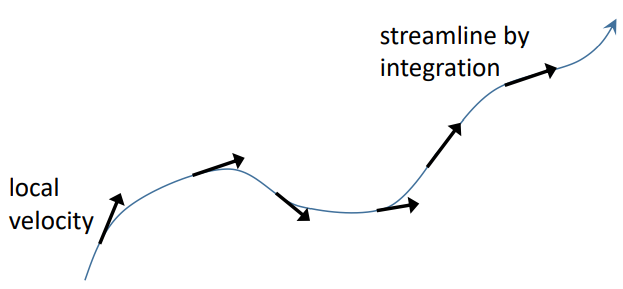
\includegraphics[width = 0.7\textwidth]{./img/diagram10.png}
    \caption{Streamline.}
\end{figure}
(note the difference from pathlines and streaklines).
\begin{itemize}[noitemsep]
    \item Streamlines do not cross (except at point source and sinks, or where mass is created or lost)
    \item They cannot meet at rigid bodies except at a special point (the stagnation point)
    \item THe surface of a body is a streamline
\end{itemize}
\section{Oblique shocks}
\subsection{Two types of oblique shock waves}
\subsubsection{Geometry controlled shocks}
This is where the deflection angle of the flow is specified.
\subsubsection{Pressure controlled shocks}
THis is where the pressure after the shock is known. Occurs in supersonic jets.
\subsection{Schematic and notation}
\begin{figure}[H]
    \centering
    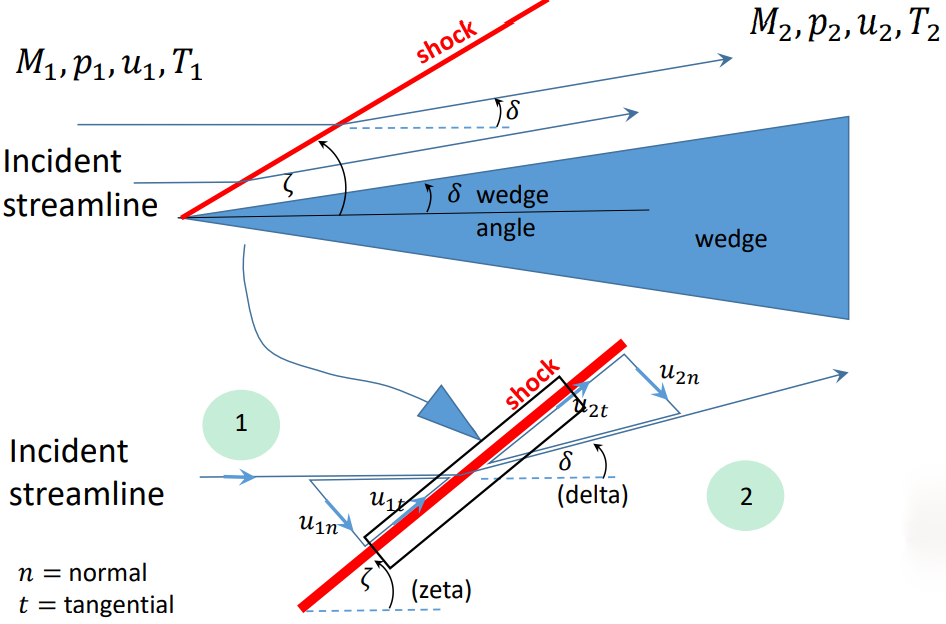
\includegraphics[width = 0.7\textwidth]{./img/diagram11.png}
    \caption{Schematic and notation.}
\end{figure}
Geometry controlled case. All angles are relative to incident streamline.
\begin{align}
    \delta & \textrm{ - deflection or wedge angle} \\
    \zeta  & \textrm{ - shock angle}
\end{align}
The aim is to relate $\delta$, $\zeta$, $M$ and $\dfrac{p_2}{p_1}$. We need to know $M_1$ and $\delta$ - geometrically constrained or $M_1$ and $\dfrac{p_2}{p_1}$ pressure constrained.
\subsection{Conservation equations}
The differential form of the conservation laws are mass:
\begin{equation}
    \underline{\nabla} \cdot \left(\rho \underline{u}\right) = 0 \textrm{ (scalar)}
\end{equation}
Momentum:
\begin{equation}
    \rho \underline{u} \cdot \underline{\nabla} \underline{u} + \underline{\nabla}p = 0 \textrm{ (vector)}
\end{equation}
Energy:
\begin{equation}
    \rho \underline{u} \cdot \underline{\nabla} \left(E + \dfrac{1}{2}q^2\right) + \underline{\nabla} \cdot \left(p \underline{u}\right) = 0
\end{equation}
The word equation form is sometimes more useful:
\begin{enumerate}[noitemsep]
    \item Mass: mass flux is conserved
    \item Momentum: increase in momentum flux is balanced by a decrease in pressure
    \item Energy: sum of internal energy and kinetic energy is equal to the work done by press.
\end{enumerate}
\subsection{Normal shock relations}
\begin{align}
    \rho_2 u_{2n}                                                   & = \rho_1 u_{1n}                                                   \\
    \rho_2 u^2_{2n} + p_2                                           & = \rho_1 u^2_{1n} + p_1                                           \\
    \frac{\gamma}{\gamma - 1}\frac{p_2}{\rho_2} + \frac{1}{2} q^2_2 & = \frac{\gamma}{\gamma - 1} \frac{p_1}{\rho_1} + \frac{1}{2}q^2_1
\end{align}
The conservation of energy is expressed in terms of the (specific) kinetic energy that depends on the gas speed $q^2 = u^2 + v^2$. As we are going to see, these relationships are identical to the oblique shock analysis.
\subsection{Oblique shock relations}
Integrating the conservation laws:
\begin{align}
    \rho_2 u_{2n}                                                                                       & = \rho_1 u_{1n}                                                                                       \\
    \rho_2 u^2_{2n} + p_2                                                                               & = \rho_1 u^2_{1n} + p_1                                                                               \\
    \frac{\gamma}{\gamma - 1}\frac{p_2}{\rho_2} + \frac{1}{2} \left(u^2_{2n} - \cancel{u^2_{2t}}\right) & = \frac{\gamma}{\gamma - 1} \frac{p_1}{\rho_1} + \frac{1}{2}\left(u^2_{1n} - \cancel{u^2_{1t}}\right)
\end{align}
The conservation of momentum tangential to the shock is:
\begin{equation}
    \rho \underline{u} \cdot \underline{\nabla}u_t = \underline{u}p \cdot\underline{\hat{t}}
\end{equation}
Where $\underline{\hat{t}}$ is the unit vector tangential to the shock. Since the pressure is constant on both sides of the shock, the RHS is zero. This means that:
\begin{equation}
    \rho_1 u_{1n}u_{1t} = \rho_2 u_{2n} u_{2t} \textrm{ or } u_{1t} = u_{2t}
\end{equation}
From the inclination of the shock and deflection angle:
\begin{align}
    u_{1n} & = u_1\sin\zeta                        \\
    u_{2n} & = u_2\sin\left(\zeta - \delta\right)  \\
    u_{1t} & = u_1 \cos \zeta                      \\
    u_{2t} & = u_2 \cos\left(\zeta - \delta\right)
\end{align}
Normal shock relationship:
\begin{equation}
    M^2_{2n} = \dfrac{1 + \frac{1}{2}\left(\gamma - 1\right)M^2_{1n}}{\gamma M^2_{1n} - \frac{1}{2}\left(\gamma -1s\right)}
\end{equation}
Oblique shock relationship:
\begin{equation}
    M^2_2 \sin^2 \left(\zeta - \delta\right) = \dfrac{1 + \frac{1}{2}\left(\gamma - 1\right)M^2_1 \sin^2\zeta}{\gamma M^2_1 \sin^2 \zeta-\frac{1}{2}\left(\gamma - 1\right)}
\end{equation}
This gives a relationship between 3 variables:
\begin{equation}
    \tan \delta = \dfrac{\cot \left(\zeta \left(M^2_1 \sin^2\left(\zeta -1\right)\right)\right)}{\frac{1}{2}\left(\gamma + 1\right)M^2_1 - M^2_1 \sin^2 \left(\zeta\right) + 1}
\end{equation}
\subsection{Relationship between $M_1$, $\zeta$ and $\delta$}
\begin{figure}[H]
    \centering
    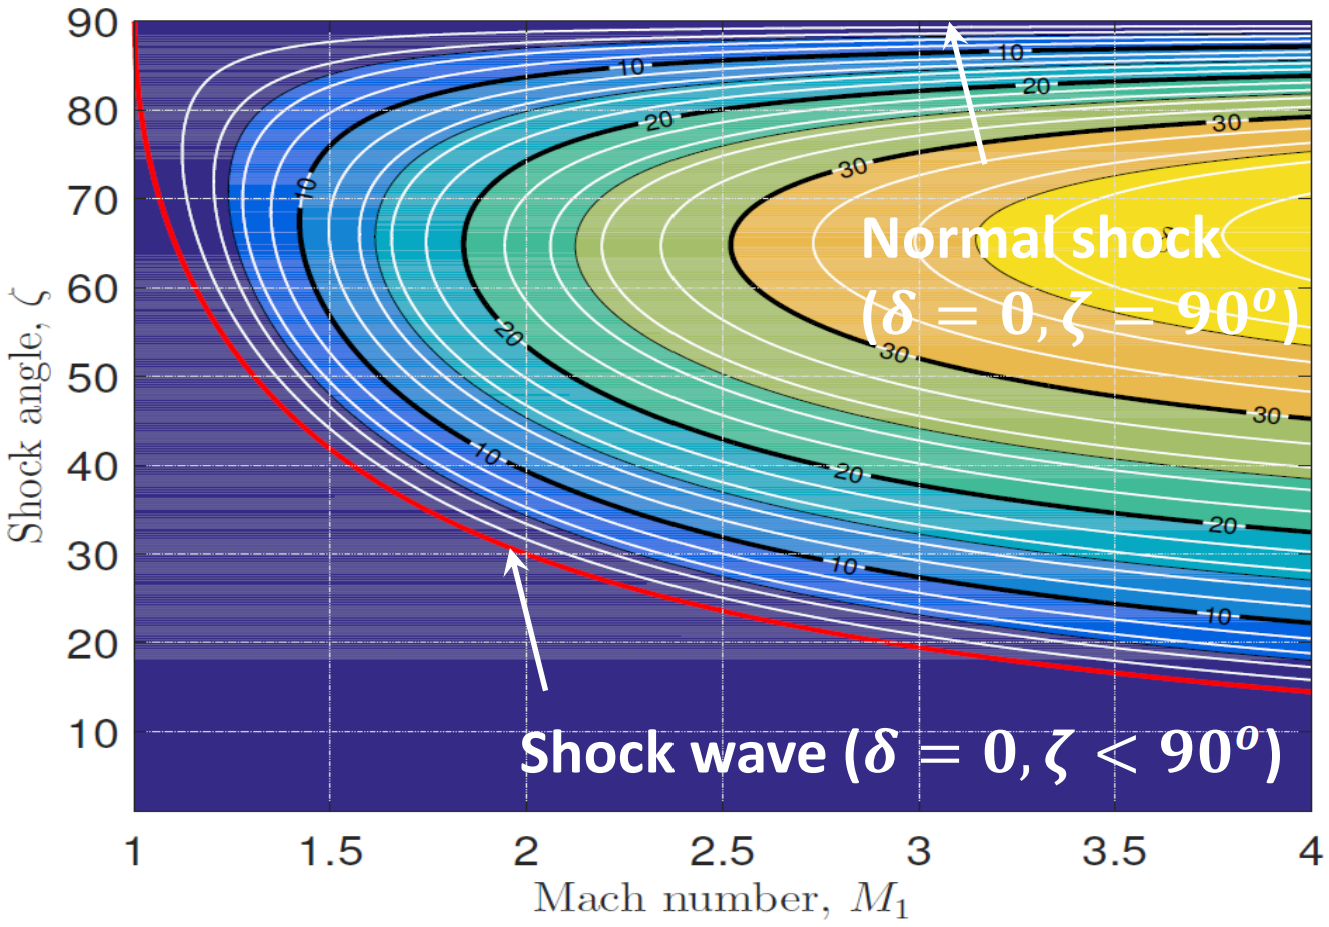
\includegraphics[width = 0.75\textwidth]{./img/diagram12.png}
    \caption{Shock angle vs Mach number.}
\end{figure}
We deconstruct the solution into parts that we can understand before looking at more specifically the solutions. For $\delta = 0$ (no streamline deflection), we have:
\begin{itemize}[noitemsep]
    \item $\zeta = \SI{90}{\degree}$: normal shock
    \item $\zeta < \SI{90}{\degree}$: shock wave
\end{itemize}
\subsection{Sonic waves}
\begin{figure}[H]
    \centering
    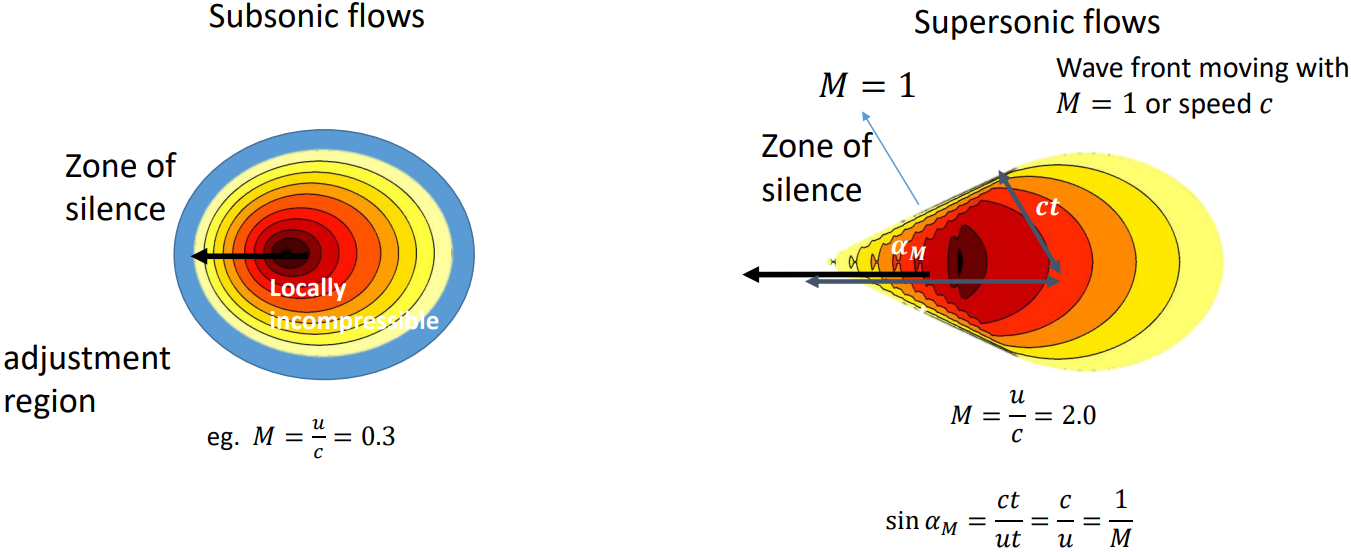
\includegraphics[width = \textwidth]{./img/diagram13.png}
    \caption{Subsonic vs supersonic flows.}
\end{figure}
\subsection{Multiple solutions ($\delta$, $\zeta$, $M_1$)}
\begin{figure}[H]
    \centering
    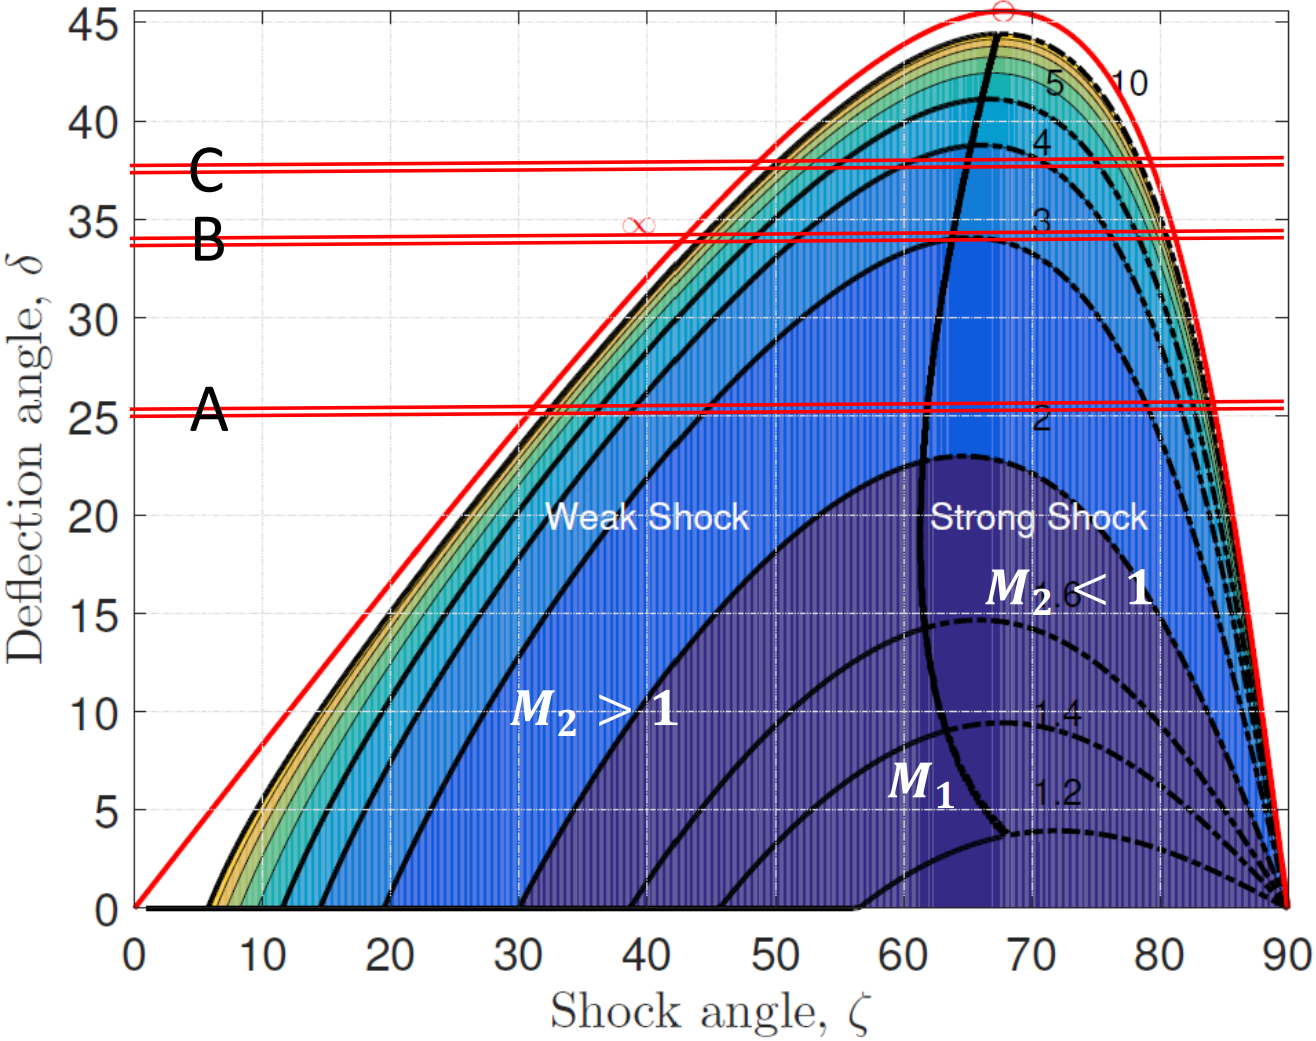
\includegraphics[width = 0.7\textwidth]{./img/diagram14.png}
    \caption{Deflection angle vs shock angle.}
\end{figure}
Look at the case where $M_1 =3$ with three examples of $\delta =$ \SI{25}{\degree}, \SI{34}{\degree} and \SI{38}{\degree}.
\begin{itemize}[noitemsep]
    \item (A) There are two solutions here, a weak shock where $\zeta =$ \SI{45}{\degree} and \SI{78}{\degree}
    \item (B) There is one unique solution $\zeta =$ \SI{68}{\degree} for $\delta =$ \SI{34}{\degree}. At wedge angles greater than this, we have case (C)
    \item (C) There is no solution here. This is because there is no way for the flow to be able to adjust by an oblique shock. Something else happens.
\end{itemize}
\begin{figure}[H]
    \centering
    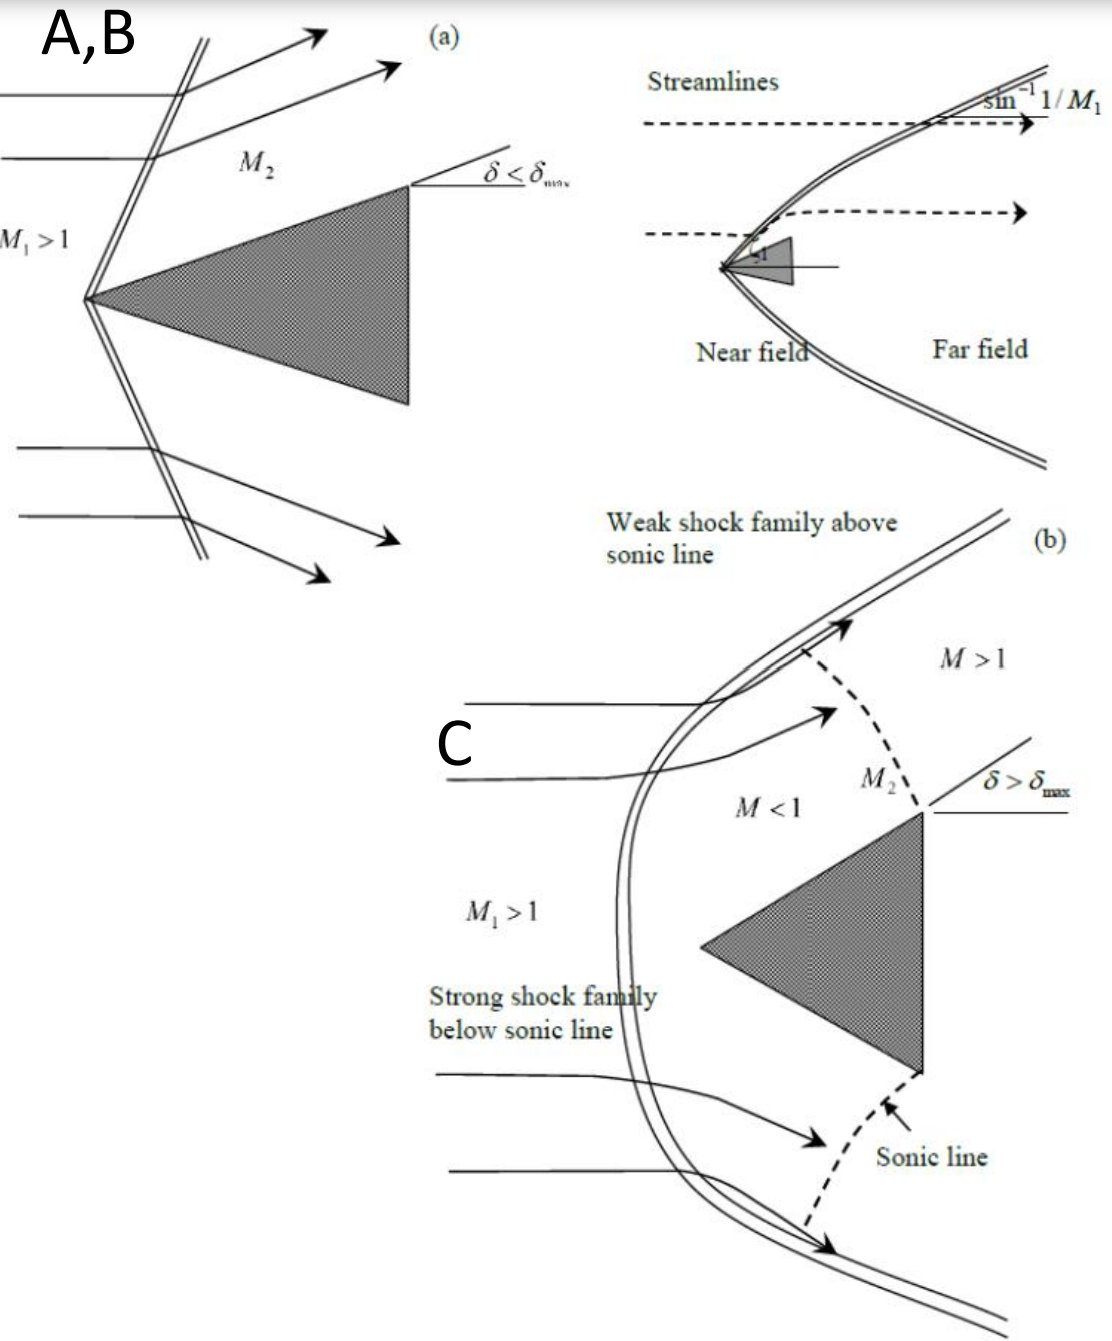
\includegraphics[width = 0.5\textwidth]{./img/diagram15.png}
    \caption{The shock angles changes from the near field to the far field.}
\end{figure}
\begin{figure}[H]
    \centering
    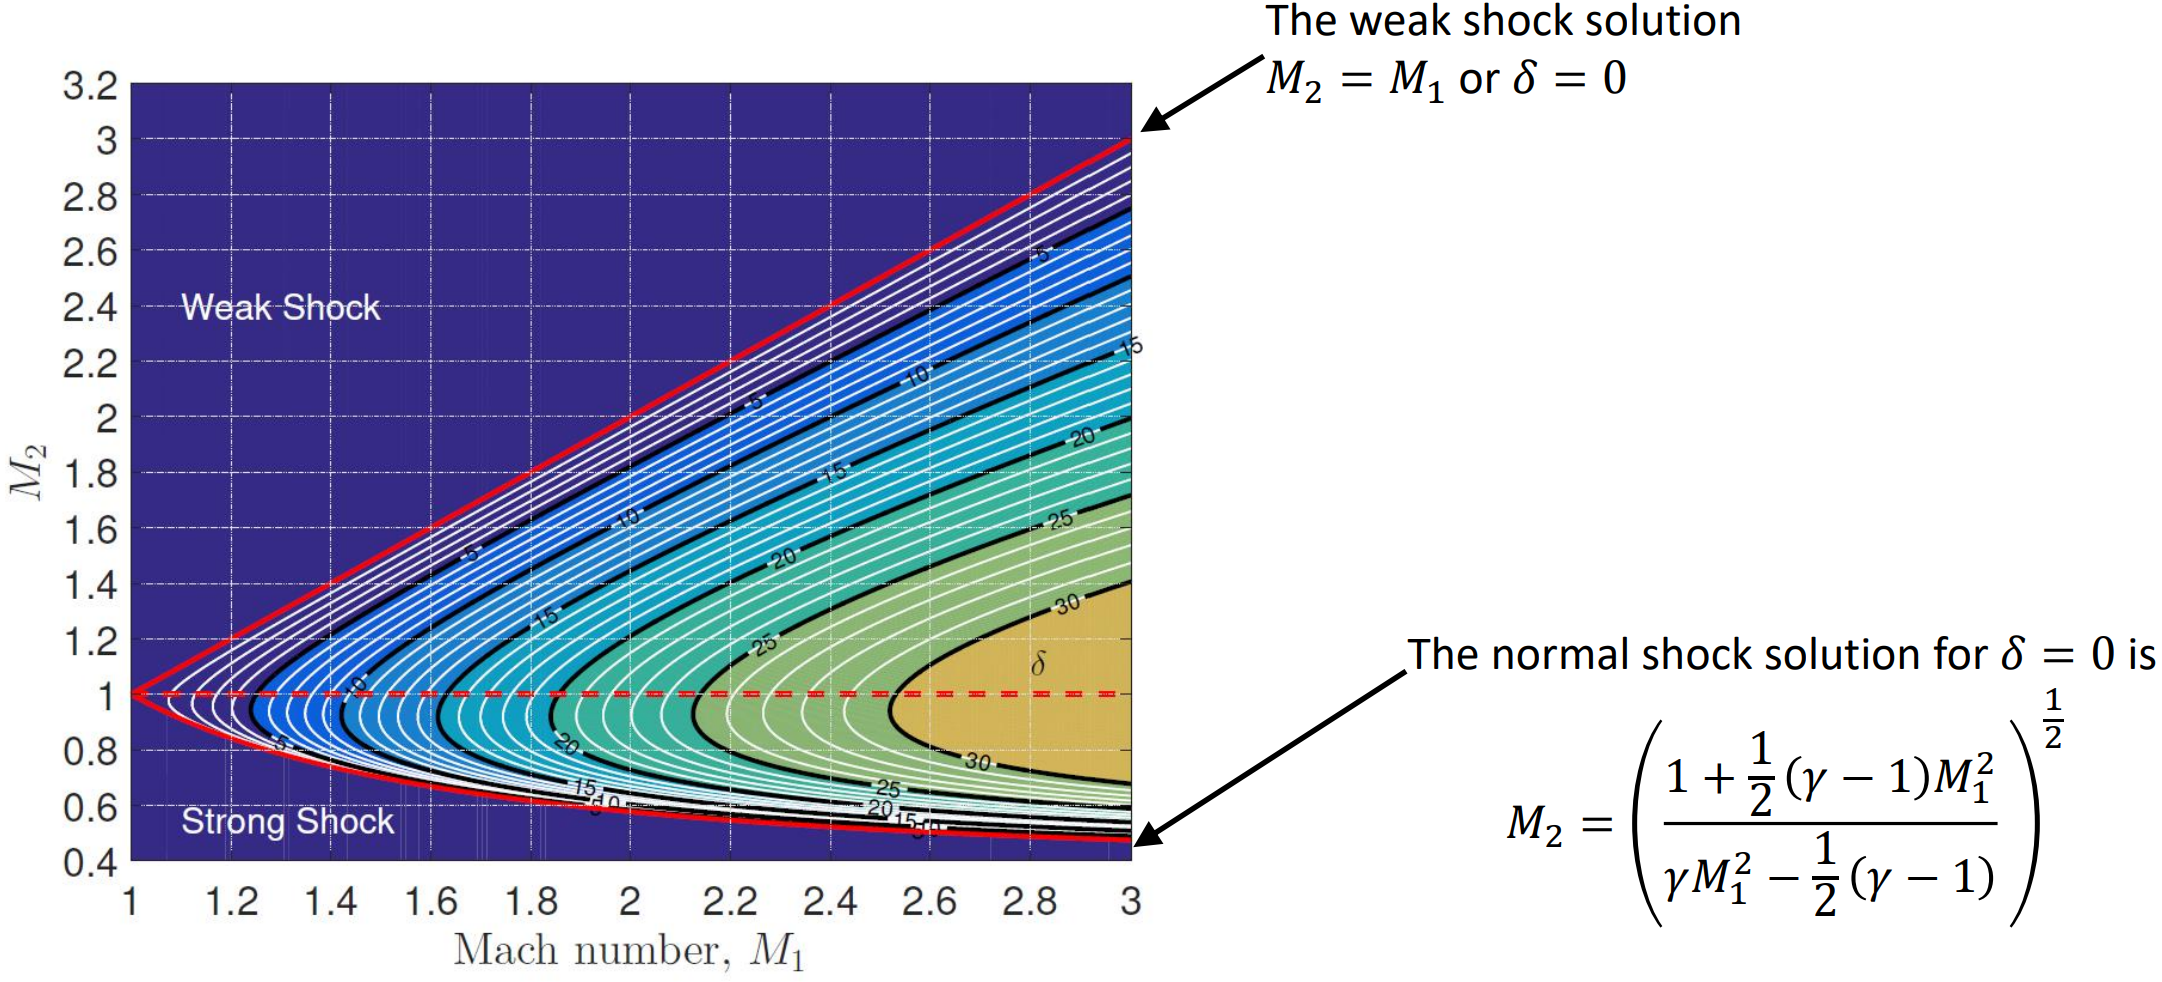
\includegraphics[width = \textwidth]{./img/diagram16.png}
    \caption{$M_2$ vs Mach number ($M_1$).}
\end{figure}
\subsection{Pressure ratio $\frac{p_2}{p_1}$}
\begin{figure}[H]
    \centering
    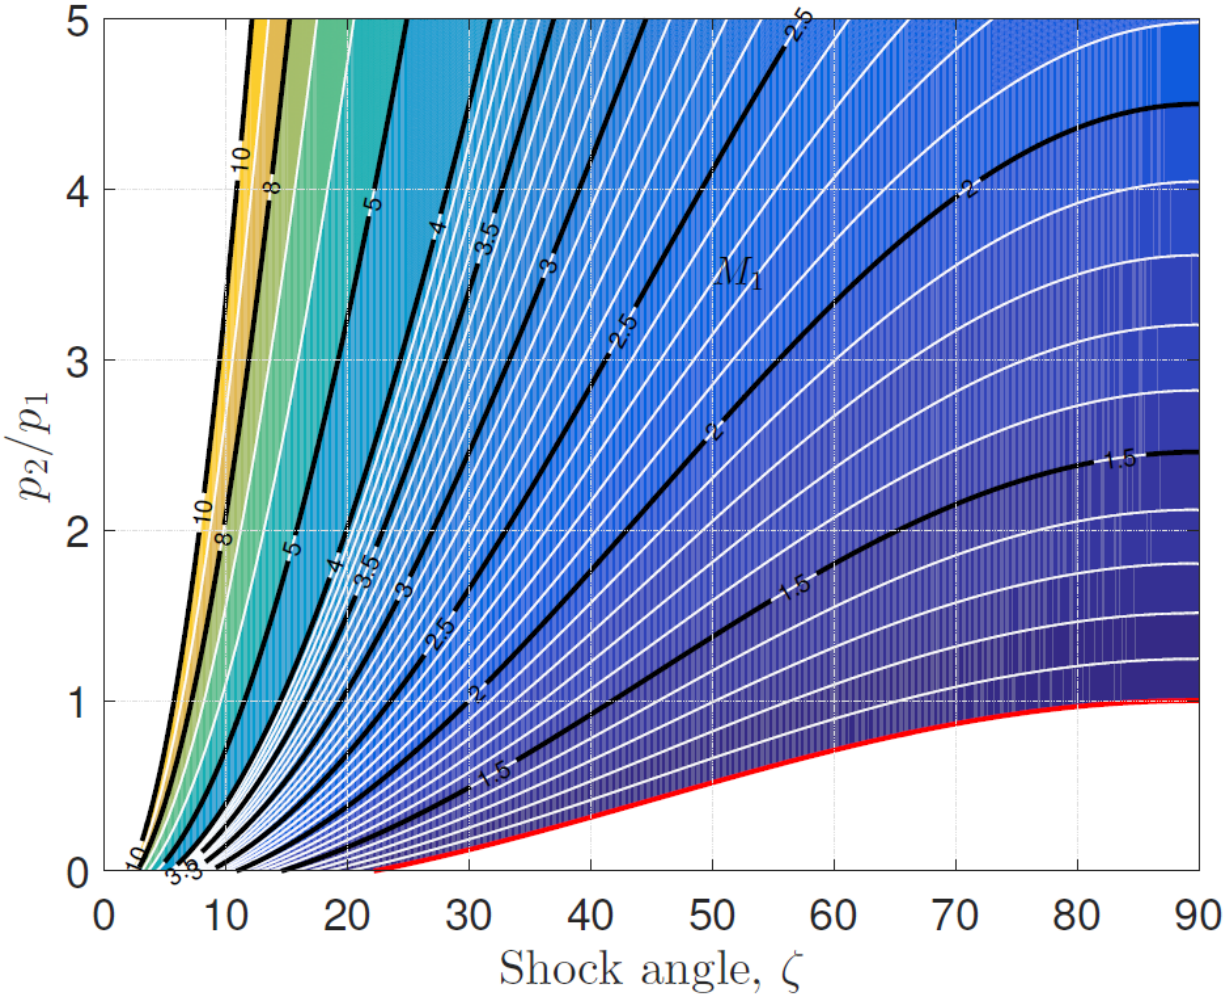
\includegraphics[width = 0.7\textwidth]{./img/diagram17.png}
    \caption{Pressure ratio vs shock angle.}
\end{figure}
The progression of the pressure across the shock is important and is calculated graphically here. Notice that in all cases, $\frac{p_2}{p_1}>1$. In the examples we have seen, the flow is controlled by the bounding geometry. In many other cases however, it is controlled by pressure, for instance, at the edge of a rocket exit.
\subsection{Summary}
Two types of shocks: geometry controlled or pressure controlled.
Two types of shocks: weak shocks and strong shocks.